\documentclass[a4j,uplatex]{jsarticle}

\usepackage[dvipdfmx]{graphicx} % 画像読み込み
\usepackage[dvipdfmx]{color} % カラー出力(色指定ができる)
\usepackage[hidelinks,bookmarksnumbered=true,dvipdfmx]{hyperref} % PDFのメタデータ埋め込み
\usepackage{pxjahyper} % しおり・タイトル等の日本語の文字化け防止
\usepackage{here} % 図表の位置を強制的に指定
\usepackage{url} % URIをそのまま表示&ハイパーリンク化

% PDFのメタデータ設定
% \hypersetup{
%   pdftitle={テスト}, %タイトル
%   pdfauthor={著者}, %著者
%   pdfsubject={VSCode環境におけるLaTeXファイルの扱いに関する研究}, %件名
%   pdfkeywords={Visual Studio Code; LaTeX;} %キーワード
% }

\begin{document}

\section{はじめに}

吾輩は猫である。名前はまだ無い。 

式\ref{eq:1}はオイラーの等式である。

\begin{equation}
  \label{eq:1}
  \mathrm{e}^{\mathrm{i}\pi} + 1 = 0
\end{equation}

画像読み込み
\begin{figure}[H]
    \centering
    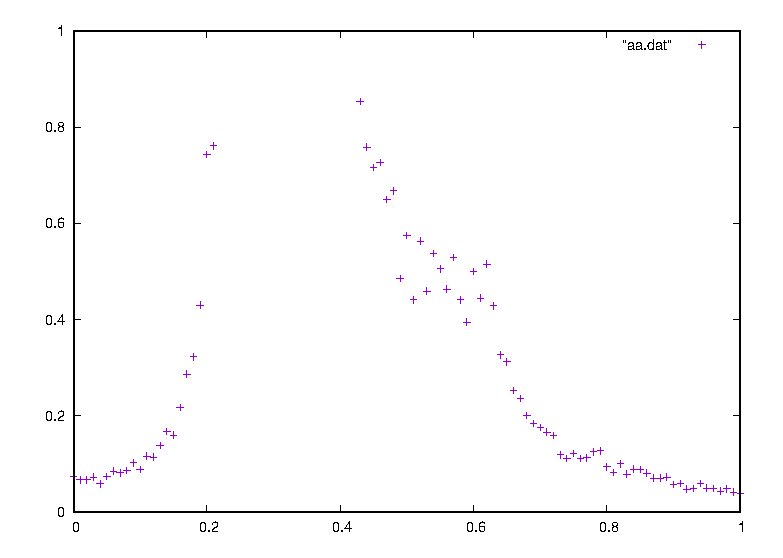
\includegraphics[height=4cm]{test.eps}
    \caption{画像}
    \label{fig:1}
\end{figure}

ほげほげ\cite{refer1}ふがふが\cite{refer2}。

% 参考文献
\begin{thebibliography}{9}
  \bibitem{refer1} 著者1, 『タイトル1』, 出版社, 出版年, pp.000-111
  \bibitem{refer2} 著者2, \url{https://www.takameron.info}, 2020年10月10日閲覧
\end{thebibliography}

\end{document}